
\documentclass[aspectratio=169]{beamer}
\usetheme{Madrid}
\usecolortheme{default}
\usefonttheme{professionalfonts}
\usepackage{amsmath,amssymb}
\usepackage{tikz}
\usetikzlibrary{positioning}
\usepackage{subcaption}
\usepackage{graphicx}
\usepackage{booktabs}
\usepackage{hyperref}
\setbeamertemplate{navigation symbols}{}
\definecolor{myblue}{RGB}{31,78,121}
\setbeamercolor{title}{fg=myblue}
\setbeamercolor{frametitle}{fg=myblue}

\title[Sybil-Robust Multi-Item Diffusion Auctions]{Sybil-Robust Multi-Item Diffusion Auctions via Cluster Reduction}
\author{Abhi Jain \and Harshit Raj \and Ridam Jan}
\institute{Course Project}
\date{April 2026}

\begin{document}

\begin{frame}
  \titlepage
\end{frame}

\begin{frame}{Problem in one line}
\begin{itemize}
    \item IDM solves truthful \emph{single-item} diffusion auctions.
    \item GIDM extends this to \emph{multiple homogeneous items}.
    \item STM/SCM make the \emph{single-item} setting Sybil-proof.
    \item \textbf{Open question:} how do we get Sybil-proofness for the multi-item case?
\end{itemize}

\vspace{0.5em}
\textbf{Our answer:} in a restricted but rigorous setting, contract Sybil clusters to certified roots and then run GIDM on the quotient graph.
\end{frame}

\begin{frame}{Flow from the baseline papers}
\centering
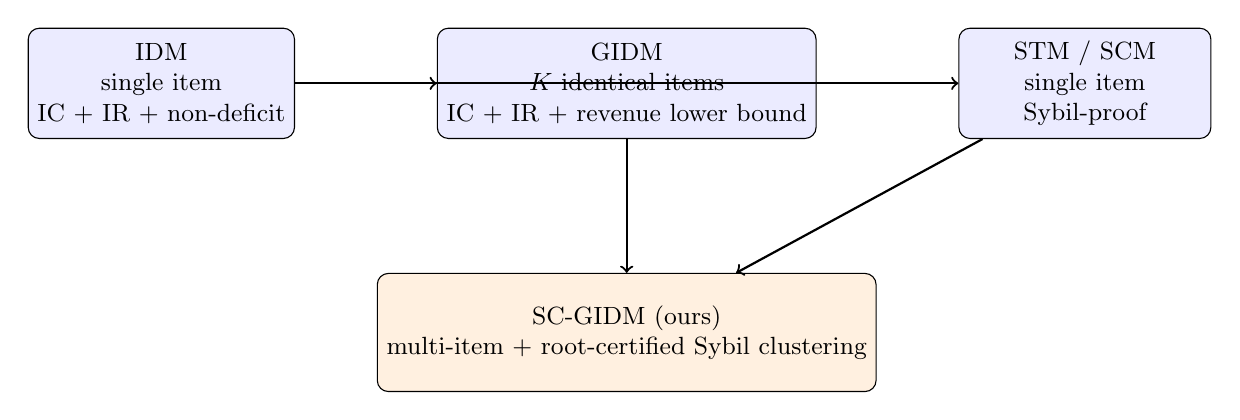
\begin{tikzpicture}[node distance=1.8cm, every node/.style={font=\small, align=center}]
\node[draw, rounded corners, fill=blue!8, minimum width=3.1cm, minimum height=1.4cm] (idm) {IDM\\single item\\IC + IR + non-deficit};
\node[draw, rounded corners, fill=blue!8, minimum width=3.2cm, minimum height=1.4cm, right=of idm] (gidm) {GIDM\\\(K\) identical items\\IC + IR + revenue lower bound};
\node[draw, rounded corners, fill=blue!8, minimum width=3.2cm, minimum height=1.4cm, right=of gidm] (scm) {STM / SCM\\single item\\Sybil-proof};
\draw[->, thick] (idm) -- (gidm);
\draw[->, thick] (idm) -- (scm);

\node[draw, rounded corners, fill=orange!12, minimum width=4.4cm, minimum height=1.5cm, below=1.7cm of gidm] (ours) {SC-GIDM (ours)\\multi-item + root-certified Sybil clustering};
\draw[->, thick] (gidm) -- (ours);
\draw[->, thick] (scm) -- (ours);
\end{tikzpicture}

\vspace{0.6em}
\begin{block}{Project philosophy}
Not ``solve everything''; solve a clean restricted version with theorem-level guarantees and experiments.
\end{block}
\end{frame}

\begin{frame}{Why naive multi-item diffusion is vulnerable}
\begin{columns}[T]
\column{0.48\textwidth}
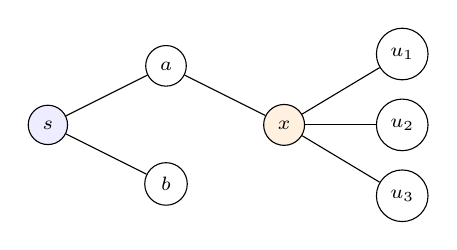
\begin{tikzpicture}[scale=0.75, every node/.style={font=\scriptsize}]
\node[draw,circle,fill=blue!7] (s) at (0,0) {$s$};
\node[draw,circle] (a) at (2,1) {$a$};
\node[draw,circle] (b) at (2,-1) {$b$};
\node[draw,circle,fill=orange!12] (x) at (4,0) {$x$};
\node[draw,circle] (u1) at (6,1.2) {$u_1$};
\node[draw,circle] (u2) at (6,0) {$u_2$};
\node[draw,circle] (u3) at (6,-1.2) {$u_3$};
\draw[-] (s)--(a); \draw[-] (s)--(b); \draw[-] (a)--(x); \draw[-] (x)--(u1); \draw[-] (x)--(u2); \draw[-] (x)--(u3);
\end{tikzpicture}

\centering Honest graph
\column{0.48\textwidth}
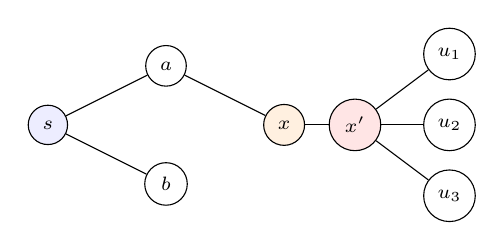
\begin{tikzpicture}[scale=0.75, every node/.style={font=\scriptsize}]
\node[draw,circle,fill=blue!7] (s) at (0,0) {$s$};
\node[draw,circle] (a) at (2,1) {$a$};
\node[draw,circle] (b) at (2,-1) {$b$};
\node[draw,circle,fill=orange!12] (x) at (4,0) {$x$};
\node[draw,circle,fill=red!10] (y) at (5.2,0) {$x'$};
\node[draw,circle] (u1) at (6.8,1.2) {$u_1$};
\node[draw,circle] (u2) at (6.8,0) {$u_2$};
\node[draw,circle] (u3) at (6.8,-1.2) {$u_3$};
\draw[-] (s)--(a); \draw[-] (s)--(b); \draw[-] (a)--(x); \draw[-] (x)--(y); \draw[-] (y)--(u1); \draw[-] (y)--(u2); \draw[-] (y)--(u3);
\end{tikzpicture}

\centering Chain Sybil attack
\end{columns}

\vspace{0.4em}
\begin{itemize}
    \item Running GIDM directly on reported identities treats fake nodes as real bidders/intermediaries.
    \item Because GIDM reduces to IDM when \(K=1\), and IDM is known to be Sybil-vulnerable, identity-level GIDM cannot be Sybil-proof in general.
\end{itemize}
\end{frame}

\begin{frame}{Our model and assumptions}
\begin{block}{Restricted setting}
\begin{itemize}
    \item \(K\) homogeneous items
    \item single-unit demand
    \item no collusion between distinct real buyers
    \item each Sybil cluster has a \textbf{certified non-Sybil root}
\end{itemize}
\end{block}

\begin{block}{Why these assumptions?}
They are exactly what makes a clean reduction proof possible.\\
We do \emph{not} claim a full detection algorithm for arbitrary Sybils.
\end{block}

\begin{alertblock}{Key design choice}
The cluster bid is the \textbf{root bid}, not the maximum Sybil bid.
\end{alertblock}
\end{frame}

\begin{frame}{Mechanism: SC-GIDM}
\begin{enumerate}
    \item Partition reported identities into Sybil clusters.
    \item Contract each cluster into one meta-buyer.
    \item Use the certified root's bid as the cluster bid.
    \item Merge all external edges into cluster-level diffusion edges.
    \item Run baseline GIDM on the quotient graph.
    \item If a cluster wins, allocate one item to its root and charge the root.
\end{enumerate}

\vspace{0.6em}
\centering
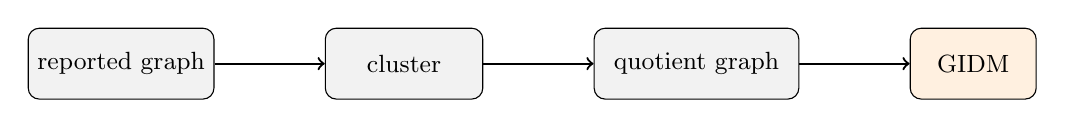
\begin{tikzpicture}[node distance=1.4cm, every node/.style={font=\small, align=center}]
\node[draw, rounded corners, fill=gray!10, minimum width=2.0cm, minimum height=0.9cm] (id) {reported graph};
\node[draw, rounded corners, fill=gray!10, minimum width=2.0cm, minimum height=0.9cm, right=of id] (cl) {cluster};
\node[draw, rounded corners, fill=gray!10, minimum width=2.6cm, minimum height=0.9cm, right=of cl] (q) {quotient graph};
\node[draw, rounded corners, fill=orange!12, minimum width=1.6cm, minimum height=0.9cm, right=of q] (g) {GIDM};
\draw[->, thick] (id)--(cl); \draw[->, thick] (cl)--(q); \draw[->, thick] (q)--(g);
\end{tikzpicture}
\end{frame}

\begin{frame}{Main theorem idea}
\small
\begin{block}{Lemma}
After cluster contraction, any Sybil attack by a real buyer \(i\) becomes a feasible \emph{single} meta-report
\[
(\widehat b_i,\widehat r_i)
\]
of the cluster root, with \(\widehat r_i \subseteq r_i\).
\end{block}

\begin{block}{Why?}
\begin{itemize}
    \item internal Sybil nodes disappear after contraction;
    \item external cluster edges can only go to true neighbours of the root;
    \item the mechanism ignores fake bids and keeps only the root bid.
\end{itemize}
\end{block}

\begin{block}{Consequence}
SC-GIDM is just GIDM on the quotient graph, so we inherit:
\[
\text{IR} + \text{IC} + \text{weak budget balance}.
\]
\end{block}
\end{frame}

\begin{frame}{Sybil-proofness theorem}
\small
\begin{theorem}
Under homogeneous items, single-unit demand, no collusion, and certified roots, SC-GIDM is Sybil-proof against identity splitting.
\end{theorem}

\begin{proof}[Proof sketch]
\begin{enumerate}
    \item Any Sybil attack collapses to a feasible deviation by one meta-buyer on the quotient graph.
    \item GIDM is truthful on that quotient graph.
    \item Cluster utility equals root utility because the cluster can receive at most one item.
    \item So creating fake identities cannot improve the real buyer's utility.
\end{enumerate}
\end{proof}

\end{frame}

\begin{frame}{Canonical profitable attack}
\begin{columns}[T]
\column{0.58\textwidth}
\begin{itemize}
    \item \(K=3\)
    \item honest GIDM winners: \(b_1,b_2,b_7\)
    \item attacker \(b_0\) utility: \(0\)
    \item attack: add one fake identity \(b_0'\) with the same bid \(98\) and place it between \(b_0\) and its neighbours
\end{itemize}

\[
p_{b_0'} = 76,\qquad p_{b_2}=-75
\]

\[
u_{b_0}^{\text{attack}} = 98 - 76 = 22
\]

\column{0.42\textwidth}
\includegraphics[width=\textwidth]{canonical_attacker_gain.png}
\end{columns}

\vspace{0.4em}
\begin{block}{What SC-GIDM does}
Cluster \( \{b_0,b_0'\} \) is contracted back to root \(b_0\), the fake bid is ignored, and the attack gain returns to \(0\).
\end{block}
\end{frame}

\begin{frame}{Simulation setup}
\begin{itemize}
    \item Graphs: random trees and connected Erd\H{o}s-R\'enyi graphs
    \item \(n=20\) real buyers, \(K=4\), \(3\) seller neighbours
    \item attacker = highest betweenness / degree buyer
    \item attack = chain Sybil attack with \(q\in\{0,1,2,3,4\}\)
    \item 120 random seeds
\end{itemize}

\vspace{0.4em}
\textbf{Compared mechanisms}
\begin{enumerate}
    \item Local-\(K\)-Vickrey
    \item honest GIDM baseline
    \item attacked GIDM
    \item SC-GIDM
\end{enumerate}
\end{frame}

\begin{frame}{Result 1: real welfare is recovered}
\begin{columns}[T]
\column{0.5\textwidth}
\includegraphics[width=\textwidth]{welfare_tree.png}
\column{0.5\textwidth}
\includegraphics[width=\textwidth]{welfare_er.png}
\end{columns}

\vspace{0.3em}
\begin{itemize}
    \item Attacked GIDM loses real welfare as \(q\) grows.
    \item SC-GIDM stays essentially on the no-attack curve.
    \item So the cluster reduction restores \emph{real} allocation quality.
\end{itemize}
\end{frame}

\begin{frame}{Result 2: fake winners disappear}
\begin{columns}[T]
\column{0.5\textwidth}
\includegraphics[width=\textwidth]{fake_winners_tree.png}
\column{0.5\textwidth}
\includegraphics[width=\textwidth]{fake_winners_er.png}
\end{columns}

\vspace{0.3em}
\begin{itemize}
    \item Ordinary attacked GIDM increasingly allocates items to fake identities.
    \item SC-GIDM eliminates fake winners because it contracts them before the auction runs.
\end{itemize}
\end{frame}

\begin{frame}{Revenue is not the whole story}
\begin{columns}[T]
\column{0.5\textwidth}
\includegraphics[width=\textwidth]{revenue_tree.png}
\column{0.5\textwidth}
\includegraphics[width=\textwidth]{revenue_er.png}
\end{columns}

\vspace{0.2em}
\begin{itemize}
    \item Fake identities can create extra competition, so attacked GIDM may show slightly higher \emph{nominal} revenue.
    \item But this comes with fake winners and lower real welfare.
    \item Therefore robustness should be evaluated by real-buyer welfare and attack-resistance, not just seller revenue.
\end{itemize}
\end{frame}

\begin{frame}{What we proved vs. what remains open}
\begin{columns}[T]
\column{0.48\textwidth}
\begin{block}{Proved}
\begin{itemize}
    \item quotient-graph reduction
    \item IR
    \item cluster-level IC
    \item weak budget balance
    \item Sybil-proofness against identity splitting
\end{itemize}
\end{block}

\column{0.48\textwidth}
\begin{alertblock}{Still open}
\begin{itemize}
    \item imperfect / heuristic Sybil detection
    \item collusion across real buyers
    \item multi-demand and heterogeneous items
    \item multiple sellers
\end{itemize}
\end{alertblock}
\end{columns}
\end{frame}

\begin{frame}{Takeaway}
\begin{block}{Main message}
A clean way to extend the single-item Sybil-proof direction to multiple items is:
\[
\text{certified Sybil clustering} \;+\; \text{GIDM on the quotient graph}.
\]
\end{block}

\begin{itemize}
    \item The mechanism is rigorous under a clear restricted model.
    \item It answers an explicit open question from the Sybil-proof paper.
    \item It works well experimentally on the metrics that matter for robustness.
\end{itemize}

\vspace{0.6em}
\centering
{\Large Thank you}
\end{frame}

\end{document}
